% convergence-rms/si30_spline_warped.tex — generated by convergence/tools/rms_figure.py; do not edit.
% One panel (Sigma 14 mm lens, Siemens stars, Spline): the median per LM iteration of the detections' true reprojection error and of the held-out reprojection error on
% the high-precision target, both in px on one axis, its key under it. The axis box is \rcpanelwidth wide (\linewidth when the host
% does not define it) and is ALL of the picture's width (trim axis left / right): the y tick labels and the y label \rcpanelylabel
% stand out to its left, the last x tick label to its right — the host leaves room for them. The baseline is the picture's lower edge.
\providecommand{\rcpanelwidth}{\linewidth}\providecommand{\rcpanelylabel}{Median reprojection error [px]}%
\definecolor{rcdet}{HTML}{228833}\definecolor{rcchr}{HTML}{0000FF}%
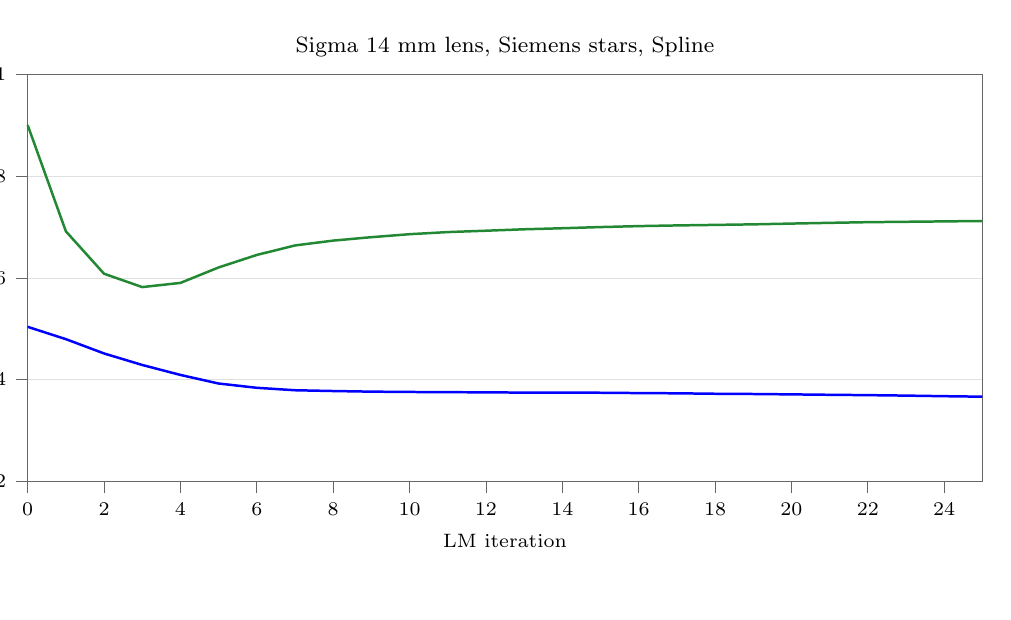
\begin{tikzpicture}[baseline=(current bounding box.south), trim axis left, trim axis right]
\begin{axis}[width=\rcpanelwidth, height=0.4259*\rcpanelwidth, scale only axis, xmin=0, xmax=25, ymin=0.2, ymax=1, ytick distance=0.2, tick label style={font=\scriptsize}, label style={font=\scriptsize}, tick align=outside, tick style={black!60, line width=0.3pt}, axis line style={black!60, line width=0.3pt}, scaled y ticks=false, title style={font=\footnotesize, yshift=-3pt}, title={Sigma 14 mm lens, Siemens stars, Spline}, xlabel={LM iteration}, xtick pos=left, ytick pos=left, ymajorgrids, grid style={black!12, line width=0.3pt}, clip=false, yticklabel style={/pgf/number format/fixed, /pgf/number format/precision=2}, ylabel={\rcpanelylabel}]
\addplot[rcchr, line width=0.9pt, no marks] coordinates {(0,0.503858) (1,0.479635) (2,0.451468) (3,0.428849) (4,0.409212) (5,0.392331) (6,0.383918) (7,0.379111) (8,0.377569) (9,0.376345) (10,0.375741) (11,0.375234) (12,0.375083) (13,0.374388) (14,0.374266) (15,0.37419) (16,0.373537) (17,0.373086) (18,0.372198) (19,0.371721) (20,0.370976) (21,0.370155) (22,0.36948) (23,0.368566) (24,0.3674) (25,0.366428)};
\addplot[rcdet, line width=0.9pt, no marks] coordinates {(0,0.900719) (1,0.691795) (2,0.608336) (3,0.582069) (4,0.590293) (5,0.620715) (6,0.645302) (7,0.663994) (8,0.673493) (9,0.680254) (10,0.686109) (11,0.690268) (12,0.692967) (13,0.695779) (14,0.697832) (15,0.700138) (16,0.702033) (17,0.703369) (18,0.704402) (19,0.705472) (20,0.70701) (21,0.708444) (22,0.709772) (23,0.710538) (24,0.711302) (25,0.712088)};
\end{axis}
% the key: centred under the axis box; it may be wider than the box, so it does not count for the picture's width (overlay) —
% the short invisible path keeps its height in the picture's bounding box
\path ([yshift=-0.5in-0.9ex]current axis.south) -- ++(0pt,2ex);
\end{tikzpicture}%
